\documentclass[9pt]{article}\usepackage[]{graphicx}\usepackage[]{xcolor}
% maxwidth is the original width if it is less than linewidth
% otherwise use linewidth (to make sure the graphics do not exceed the margin)
\makeatletter
\def\maxwidth{ %
  \ifdim\Gin@nat@width>\linewidth
    \linewidth
  \else
    \Gin@nat@width
  \fi
}
\makeatother

\definecolor{fgcolor}{rgb}{0.345, 0.345, 0.345}
\newcommand{\hlnum}[1]{\textcolor[rgb]{0.686,0.059,0.569}{#1}}%
\newcommand{\hlstr}[1]{\textcolor[rgb]{0.192,0.494,0.8}{#1}}%
\newcommand{\hlcom}[1]{\textcolor[rgb]{0.678,0.584,0.686}{\textit{#1}}}%
\newcommand{\hlopt}[1]{\textcolor[rgb]{0,0,0}{#1}}%
\newcommand{\hlstd}[1]{\textcolor[rgb]{0.345,0.345,0.345}{#1}}%
\newcommand{\hlkwa}[1]{\textcolor[rgb]{0.161,0.373,0.58}{\textbf{#1}}}%
\newcommand{\hlkwb}[1]{\textcolor[rgb]{0.69,0.353,0.396}{#1}}%
\newcommand{\hlkwc}[1]{\textcolor[rgb]{0.333,0.667,0.333}{#1}}%
\newcommand{\hlkwd}[1]{\textcolor[rgb]{0.737,0.353,0.396}{\textbf{#1}}}%
\let\hlipl\hlkwb

\usepackage{framed}
\makeatletter
\newenvironment{kframe}{%
 \def\at@end@of@kframe{}%
 \ifinner\ifhmode%
  \def\at@end@of@kframe{\end{minipage}}%
  \begin{minipage}{\columnwidth}%
 \fi\fi%
 \def\FrameCommand##1{\hskip\@totalleftmargin \hskip-\fboxsep
 \colorbox{shadecolor}{##1}\hskip-\fboxsep
     % There is no \\@totalrightmargin, so:
     \hskip-\linewidth \hskip-\@totalleftmargin \hskip\columnwidth}%
 \MakeFramed {\advance\hsize-\width
   \@totalleftmargin\z@ \linewidth\hsize
   \@setminipage}}%
 {\par\unskip\endMakeFramed%
 \at@end@of@kframe}
\makeatother

\definecolor{shadecolor}{rgb}{.97, .97, .97}
\definecolor{messagecolor}{rgb}{0, 0, 0}
\definecolor{warningcolor}{rgb}{1, 0, 1}
\definecolor{errorcolor}{rgb}{1, 0, 0}
\newenvironment{knitrout}{}{} % an empty environment to be redefined in TeX

\usepackage{alltt}
\usepackage{amsmath}
\usepackage{graphicx,psfrag,epsf}
\usepackage{enumerate}
\usepackage{natbib}
\usepackage[colorlinks=true,linkcolor={blue},citecolor={blue},urlcolor={blue}]{hyperref}
\usepackage{longtable,ctable}
\usepackage{amssymb}
\usepackage{amsfonts}
\usepackage{multirow}
\usepackage{graphicx}
\usepackage{booktabs}
\usepackage{mathptmx}
\usepackage{setspace}
\usepackage[utf8]{inputenc}
\usepackage{pgf}
\usepackage{algorithm}
\usepackage{algpseudocode}
\usepackage{threeparttable}
\usepackage{verbatim}
\usepackage{bm}
\usepackage{xcolor}



%\pdfminorversion=4
% NOTE: To produce blinded version, replace "0" with "1" below.
\newcommand{\blind}{0}

% DON'T change margins - should be 1 inch all around.
\addtolength{\oddsidemargin}{-.5in}%
\addtolength{\evensidemargin}{-.5in}%
\addtolength{\textwidth}{1in}%
\addtolength{\textheight}{1.3in}%
\addtolength{\topmargin}{-.8in}%


\newcommand{\R}{R}
\newcommand{\gbsg}{gbsg}
\def\FsNg{\hbox{FS-M}}

\def\hhat{\hat\theta(\widehat{H})}
\def\hchat{\hat\theta(\widehat{H}^{c})}

\def\hhatB{\hat\theta^{*}(\widehat{H})}
\def\hchatB{\hat\theta^{*}(\widehat{H}^{c})}


\def\hknow{\hat\theta(H)}
\def\hcknow{\hat\theta(H^{c})}

\def\hplim{\theta^{\dagger}(H)}
\def\hcplim{\theta^{\dagger}(H^{c})}
\def\hplimitt{\theta^{\dagger}(ITT)}

\def\fsl{FS_{l}}
\def\fslg{FS_{lg}}
\def\grfa{GRF}
\def\grfb{GRF_{60}}


\def\hhplim{\theta^{\ddagger}(H)}
\def\hhcplim{\theta^{\ddagger}(H^{c})}

\def\Hhplim{\theta^{\ddagger}(\widehat{H})}
\def\Hhcplim{\theta^{\ddagger}(\widehat{H}^{c})}

\def\hath{\widehat{H}}
\def\hathc{{\widehat{H}}^{c}}


\def\sumin{\sum_{i=1}^n}
\def\nsumin{n^{-1}\sum_{i=1}^n}

\newcommand{\indep}{\perp \!\!\! \perp}
\IfFileExists{upquote.sty}{\usepackage{upquote}}{}
\begin{document}

\def\spacingset#1{\renewcommand{\baselinestretch}%
{#1}\small\normalsize} \spacingset{1}


\if0\blind
{
  \title{\bf Exploratory subgroup identification in the heterogeneous Cox model: A relatively simple procedure}
  \date{}
  \author{Larry F. Le\'on %\thanks{}\hspace{.2cm}
  , Thomas Jemielita, \\ Zifang Guo, Rachel Marceau West, and Keaven Anderson \\
    Biostatistics and Research Decision Sciences, Merck \& Co., Inc., Rahway, NJ, USA}
  \maketitle
} \fi


\bigskip
\begin{center}
{\large\bf SUPPLEMENTARY MATERIALS}
\end{center}

Section S1.1 considers the accuracy of the $N(\beta,8/d)$ asymptotic approximation to the random splits of the FS algorithm where the sample size is $N=60$.  Section S2.1 provides an 
additional analysis of the GBSG dataset. Section S2.2 provides an additional analysis of the ACTG-175 dataset.  Sections S2.3 and S2.4 provide additional analyses of the ACTG-175 dataset
where we artificially add twenty $N(0,1)$ baseline factors as candidates: In Section S2.3 the FS algorithm does not include lasso, whereas in Section S2.4 lasso is included.  Section S2.5 evaluates 
the use of aspirin in the systolic heart failure data (\citealp{Hsich_2011}) available in the \verb+randomForestSRC+ package (\citealp{Ishwaran_2008}).  Lastly, in Section S3 we 
apply the subgroup definitions based on the GBSG analysis to the Rotterdam data \citep{Foekens_2000} which was utilized for ``external validation of a Cox prognostic model'' \citep{Royston_2013}.

R code and markdown files for replicating the analyses is available at the GitHub repository: \href{https://github.com/larry-leon/forestSearch}{https://github.com/larry-leon/forestSearch}. 
We note that an R package to be published on CRAN is under development.  Our code implements parallel computing via the \verb+doFuture+ package (\citealp{Bengtsson_2021}) for the bootstrapping and CV procedures; accordingly the timing of computations depends on the number of available cores.






\section*{S1 Power approximations}


\section*{S1.1 Simulation evaluation of $\hat\beta \sim N(\beta,4/d)$ approximation accuracy} \label{sec:Napprox}

For the random splitting of the FS algorithm we approximate the separate splits via $\hat\beta_{s}^{1} \sim N(\beta,8/d)$ and independently $\hat\beta_{s}^{2} \sim N(\beta,8/d)$.  Define
$\hat\beta_{s}$ as the Cox model estimate for the subgroup.  Since the splits are purely random (the artificially stratified Cox model estimate will be approximately the same as $\hat\beta_{s}$) we have 
$\hat\beta_{s}^{1} + \hat\beta_{s}^{2} \approx 2 \hat\beta_{s}$.

Figure \ref{fig:Napprox} is based on 20,000 simulations where we generate $N=60$ subjects from a Cox model with (true) $\beta \approx -0.4$ with number of events (on average) $=31.9$.
Figure \ref{fig:Napprox}(a) plots the empirical cdf (ECDF) of the 20,000 estimates corresponding to the first split ($\hat\beta_{s}^{1}$) along with the $N(\beta,8/d)$ approximation.  Similarly, 
Figure \ref{fig:Napprox}(b) displays the results for the corresponding second split ($\hat\beta_{s}^{2}$).   Figure \ref{fig:Napprox}(c) plots the ECDF of 20,000 $(\hat\beta_{s}^{1} + \hat\beta_{s}^{2})$'s, along with the ECDF of 20,000 $2\hat\beta_{s}$'s.  Figure \ref{fig:Napprox}(d) plots the ECDF of 20,000 $\min(\hat\beta_{s}^{1},\hat\beta_{s}^{2})$'s along with the $1-(1-N(\beta,8/d)^{2})$ approximation.

\begin{figure}[h]
\begin{center}
\begin{knitrout}
\definecolor{shadecolor}{rgb}{0.969, 0.969, 0.969}\color{fgcolor}
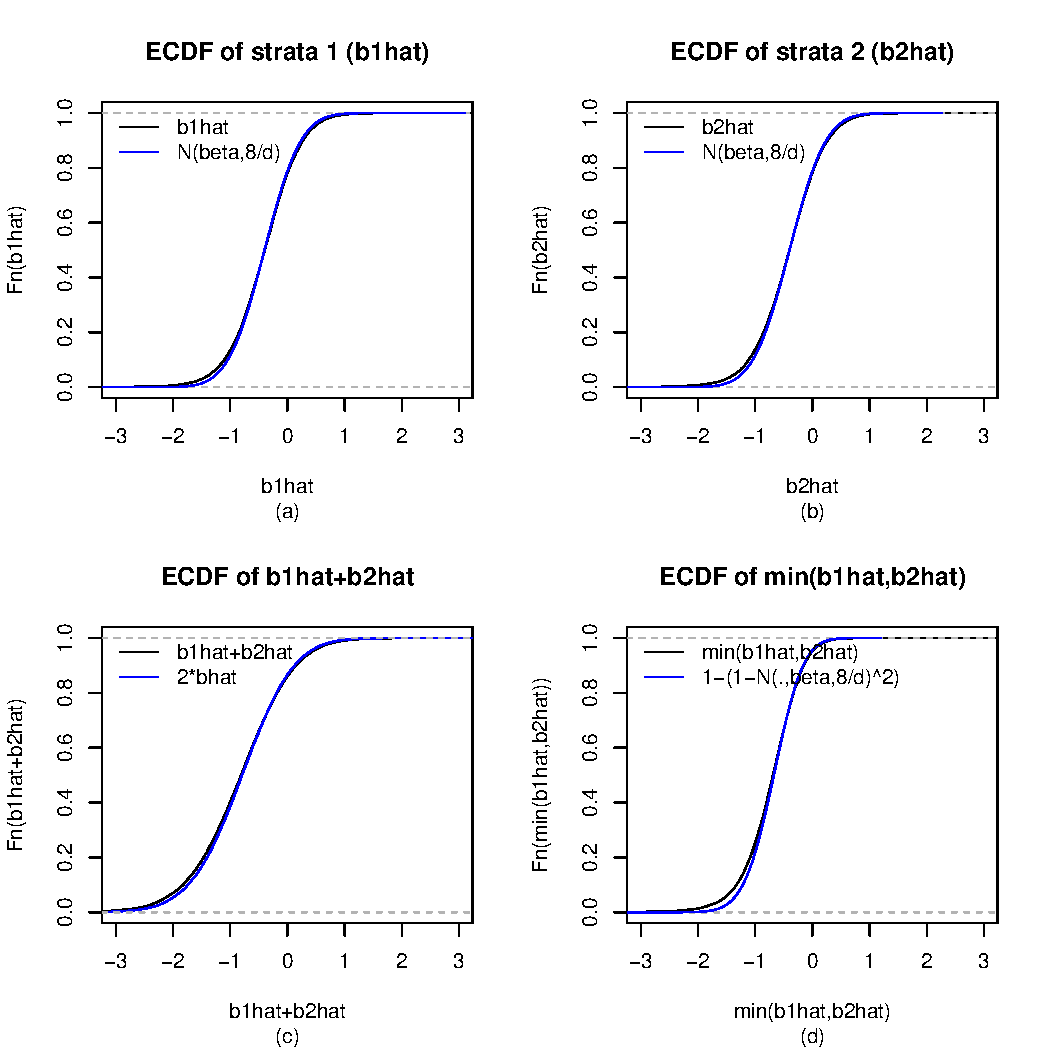
\includegraphics[width=\maxwidth]{figure/sim_approxH-S1-1} 
\end{knitrout}
\end{center}
\caption{Accuracy of normal approximation $\hat\beta \approx N(\beta,8/d)$}
\label{fig:Napprox}
\end{figure}


\section*{S1.2 Power approximations for censoring rates of $0\%$ and $80\%$}





\begin{figure*}
\begin{center}
\includegraphics[width=5.5in, height=3.25in]{plot_approxH_nocensoring.pdf}
\end{center}
\caption{Approximate probability of finding H via FS: Subgroup $H$ of size $n=60, 80, 100$ exists with underlying hazard-ratio varying from 0.5 to 3.0 and with assumed average censoring rate of $0\%$ so that $d = n$.  The horizontal line indicates $10\%$. Approximately $80\%$ reached at underlying hazard-ratios of $1.69$, $1.6$, and $1.56$, for $n$ = 60, 80, and 100, respectively. \label{fig:ApproxH_nocensoring}}
\end{figure*}

Figure {\ref{fig:ApproxH_nocensoring}} displays the approximate power under no censoring for scenarios where a subgroup $H$ exists ($n=$ 60, 80, or 100) with underlying hazard-ratio for subgroup $H$ varying from $0.5$ to $3.0$.
For $\hplim \equiv \hplimitt = 0.75$, the approximation is $0.018$, $0.009$, and $0.004$ for $n=60$, $80$, and $100$, respectively.





\begin{figure*}
\begin{center}
\includegraphics[width=5.5in, height=3.25in]{plot_approxH_heavycensoring.pdf}
\end{center}
\caption{Approximate probability of finding H via FS: Subgroup $H$ of size $n=60, 80, 100$ exists with underlying hazard-ratio varying from 0.5 to 3.0 and with assumed average censoring rate of $80\%$ so that $d \approx 0.20n$.  The horizontal line indicates $10\%$. Approximately $80\%$ reached at underlying hazard-ratios of $2.83$, $2.49$, and $2.28$, for $n$ = 60, 80, and 100, respectively. \label{fig:ApproxH_heavycensoring}}
\end{figure*}

Figure {\ref{fig:ApproxH_heavycensoring}} displays the approximate power under heavy censoring of $80\%$ for scenarios where a subgroup $H$ exists ($n=$ 60, 80, or 100).
Here, for $\hplim \equiv \hplimitt = 0.75$, the approximation is $0.114$, $0.096$, and $0.081$ for $n=60$, $80$, and $100$, respectively.  However, note that these calculations do not take into account the $d \geq 20$ requirement of the FS procedure which would not be generally met for subgroup sample sizes of $60$ and $80$, here.


\section*{S2 Additional analyses}

















\begin{figure}
\begin{center}
\includegraphics[width=\textwidth, height=3.25in]{plot_KM_gbsg_supplementary.pdf}
\end{center}
\caption{GBSG analysis application of Forest Search. Kaplan-Meier (K-M) curves (un-adjusted for the estimation of subgroups): (a) Forest Search $\widehat{H}$ subgroup treatment estimates;
(b) Forest Search $\widehat{H}^{c}$ subgroup K-M treatment estimates.}
\label{fig:gbsgSupp}
\end{figure}


\subsection*{S2.1 GBSG Analysis}

We consider an alternative analysis of the German Breast Cancer Study Group trial data \citep{Schumacher_1994}.   In the analysis of the main text we
employed the selection criterion where the largest subgroup achieving a consistency rate of at least $90\%$ is chosen based on a broad set of candidate baseline factor cuts.  Here we consider the FS 
criterion of maximizing the consistency rate where lasso is utilized in conjunction with GRF (in a less broad manner in comparison to the main text).  Recall the study sample size was $N=686$ and the observed censoring rate was $\approx 56\%$.  The Cox ITT HR estimate (with only treatment as covariate) is $0.69$ ($0.54$, $0.89$).
There were seven prognostic factors collected: \verb+Estrogen+, \verb+Age+, \verb+Prog+, \verb+Meno+, \verb+Nodes+, \verb+Size+, and \verb+Grade+.   The factors \verb+Meno+ and \verb+Grade+ (\verb+Grade+ defined as grade 1/2 vs 3) are categorical and the rest are continuous. 
The first stage of our algorithm is to apply lasso which selects \verb+Size+, \verb+Grade+, \verb+Nodes+, and \verb+Prog+.  Applying GRF ($\grfb$ with a 6-month RMST criterion) selects \verb+Estrogen<=0+.  Now, the analyses of \cite{Sauerbrei_1999} suggest that \verb+Age+ 
may be prognostic with inflection points at 40 and 55 years (See their Figure 2).  We therefore consider these two cuts as candidates (``forced as candidates'' regardless of lasso and GRF).  In summary, we consider seven candidate factors:  \verb+Size<=median(Size)+; \verb+Nodes<=median(Nodes)+; \verb+Prog<=median(Prog)+; 
\verb+Estrogen<=0+; \verb+Age<=40+; \verb+Age<=55+; and \verb+Grade+.  There are then $L = 14$ total single factor subgroups with $L*(L-1)/2+L = 105$ possible subgroups (two-factor combinations):  Among these 
subgroups the number of candidates with sample sizes $\geq 60$ and at least $10$ events in each arm is reduced to $68$. 

 The $\fslg$ approach, maximizing consistency, estimates $\widehat{H}$ as the subgroup formed by the combination of \verb+Estrogen<=0+ and \verb+Prog<=32.5+ (The consistency rate is $98.9\%$).  That is, $\widehat{H}$ subjects are those with an estrogen level of $0$ and progesterone values at or 
 below $32.5$ ($n= 75$).  The resulting $\hat{H}$-estimates are $\hhat = 2.22$ ($1.18$, $4.2$) and (bootstrap bias-corrected) $\hhatB =1.59$ ($0.82$, $3.11$).  For the complement, $\hchat = 0.61$ ($0.46$, $0.79$) and $\hchatB =0.62$ ($0.42$, $0.9$).  Figure \ref{fig:gbsgSupp} displays the Kaplan-Meier curves for the estimated subgroups.

To evaluate the quality and stability of the subgroup selection algorithm we apply $N$-fold and 10-fold cross-validation as described in the main text.  Recall for $N$-fold 
cross validation we exclude each subject from the analysis and predict their $\widehat{H}$ ($\widehat{H}^{c}$) classification (based on the remaining $n-1$ subjects) where if a subgroup 
is not identified then the subject is classified as $\widehat{H}^{c}$ (i.e., $\widehat{H}= \emptyset$).   In contrast, for 10-fold cross-validation we randomly partition the data into 10 folds and for each fold select $\widehat{H}$ based on the 
remaining 9 folds to predict the classification for the left out fold.  Since this depends on the random partition we repeat this $200$ 
times.

For the $N$-fold cross-validation, across the $n=686$ training sets (based on deleting a single subject) there were 622 ($91$\%) subgroups identified wherein \verb+Estrogen<=0+ is selected 621 times and \verb+Prog<=32+ and \verb+Prog<=33+ are selected 342 and 260 times (resp.).  Approximately $9$\% of the subjects are classified as ITT:=$\widehat{H}^{c}$ due to lack of subgroup identification and in total $n=40$ subjects ($N$-fold predicted) are classified as $\widehat{H}$ (in contrast to $n=75$ for the full analysis).
Despite the seemingly reasonable agreement between the identified subgroup definitions, the Cox model estimate for the $N$-fold predicted subgroup $\widehat{H}$ is $0.26$ ($0.08, 0.90$) which dramatically differs from the full analysis $\hhatB =1.59$ ($0.82$, $3.11$).  In addition, across $200$ random 10-fold cross-validation analyses the median number of training sets where a subgroup was identified was only 6 out of 10 resulting in a low (median) sensitivity of $sens(\widehat{H}) = 52\%$.  That is, among the $\widehat{H}$-classified subjects based on the full analysis the median percentage also $\widehat{H}$-classified in the (10-fold) cross-validation testing samples is approximately only $50\%$.

In comparison to the analysis of the main text, the FS criterion of maximizing the consistency rate where candidate factors are selected in the above manner does not appear to 
exhibit preferable stability properties for this data application.










  

  
  

  



\begin{figure}
\begin{center}
\includegraphics[width=\textwidth, height=3.25in]{plot_KM_actg_supplementary.pdf}
\end{center}
\caption{ACTG-175 analysis application of Forest Search. Kaplan-Meier (K-M) curves (un-adjusted for the estimation of subgroups): (a) Forest Search $\widehat{Q}$ subgroup treatment estimates;
(b) Forest Search $\widehat{Q}^{c}$ subgroup K-M treatment estimates.}
\label{fig:KM_actg1}
\end{figure}

\subsection*{S2.2 ACTG-175 Analysis}

We now consider additional analyses of the AIDS Clinical Trials Group Protocol 175 study (\citealp{ACTG175}) where, as in the main text, 
the goal is to identify whether a subgroup exists with a pronounced treatment benefit.  Recall we consider the following fifteen baseline covariates: \verb+Age+, \verb+Wtkg+, \verb+Karnof+ (Karnofsky score), \verb+Cd40+, \verb+Cd80+, \verb+Hemo+ (hemophilia), \verb+HA+ (homosexual activity), 
\verb+Drugs+ (history of IV drug use), \verb+Race+, \verb+Gender+, \verb+Oprior+ (prior anti-viral therapy), \verb+Symptom+, 
\verb+Preanti+ (days prior antiretroviral therapy), \verb+Str2+ (0=naive antiretroviral history,1=experienced), and \verb+Z30+ (zidovudine 30 days prior to study). 

In contrast to the analysis of the main text, here we only consider cuts for continuous factors at the mean or median.  Briefly, the lasso and GRF algorithms lead to the following candidate factors: \verb+Cd40+, \verb+Cd80+, and \verb+Age+ are cut at the medians; \verb+Wtkg<=68.04+, \verb+Age<=29+, \verb+Preanti<=406+, \verb+Karnof<=mean+, \verb+HA+, and \verb+Symptom+ are also included.  Here the mean cut for \verb+Karnof+ and median for \verb+Age+ were ``forced'' as candidates.  Note that the median for \verb+Karnof+ is also the maximum and thus a cut at the median is not viable; And for \verb+Age+, the median (= 34 years) is forced as a candidate since the results of \cite{CZ_2023} suggest an inflection point for age between 30 and 40 years (See their Figure 4).

There are then $L = 18$ total single factor subgroups with $L*(L-1)/2+L = 171$ possible subgroups:  Among these 
subgroups the number of candidates with sample sizes $\geq 60$ and at least $10$ events in each arm is reduced to $151$. The largest subgroup with a consistency 
rate of at least $90\%$ is the subgroup formed by the combination of \verb+Preanti <= 406+ and \verb+Age > 34+ ($98.3\%$).  The resulting $\widehat{Q}$-estimates are $\hat\theta(\widehat{Q}) = 0.4$ ($0.22$, $0.73$) and (bootstrap bias-corrected) 
$\hat\theta^{*}(\widehat{Q}) =0.48$ ($0.27$, $0.85$).  For the complement, $\hat\theta(\widehat{Q}^{c}) = 1.05$ ($0.78$, $1.4$) and $\hat\theta^{*}(\widehat{Q}^{c}) =0.98$ ($0.67$, $1.43$). Figure \ref{fig:KM_actg1} displays the Kaplan-Meier curves for the estimated subgroups.


For the $N$-fold cross-validation, across the $n=1083$ training sets there were 
$1069$ ($98.7\%$) subgroups identified wherein the full analysis subgroup $\widehat{Q}$ 
definitions, \verb+Preanti<=406+ and \verb+Age>34+, are reproduced for all (except 1). A total of    
$14$ ($1$\%) subjects were classified as ITT:=$\widehat{Q}^{c}$ due to lack of subgroup identification and in total $n=309$ subjects ($N$-fold predicted) are classified as $\widehat{Q}$ (versus $n=310$ for the full analysis). 
The Cox model estimate for the $N$-fold predicted subgroup $\widehat{Q}$ is $0.45$ [$95\%= 0.25, 0.81$] which is similar 
to the (bootstrap bias-adjusted) full analysis $\hat\theta^{*}(\widehat{Q}) =0.48$ ($0.27$, $0.85$); And for the complement, the $N$-fold predicted subgroup $\widehat{Q}^{c}$ is $1.01$ ($0.76, 1.36$) which is similar 
to the full analysis $\hat\theta^{*}(\widehat{Q}^{c}) =0.98$ ($0.67$, $1.43$).

Across $200$ random 10-fold cross-validation analyses the median number of training sets (10 folds) where a subgroup was identified was only 6 out of 10 (The minimum was 3/10 with lower and upper quartiles of 6/10 and 7/10, resp.) resulting in a low (median) sensitivity of 
$sensCV(\widehat{Q}) = 50\%$.  That is, among the $\widehat{Q}$-classified subjects based on the full analysis the median percentage also $\widehat{Q}$-classified in the (10-fold) cross-validation testing samples is approximately only $50\%$.  The median positive predictive value was 
$ppvCV(\widehat{Q}) \approx 69\%$. For the complement $\widehat{Q}^{c}$, the medians for $sensCV$ and $ppvCV$ were $91\%$ and $82\%$, respectively.  In addition, across the $200$ random 10-fold cross-validation analyses, the exact $\hat{Q}$ subgroup definition of \verb+Preanti<=406+ and \verb+Age>34+ was exactly reproduced $20\%$ of the time (median), while definitions based on (cuts of) \verb+Preanti+ and \verb+Age+ appeared (a median of) $40\%$ and $50\%$ of the time, respectively (and jointly $40\%$).   Although the subgroup estimates are similar to the analysis of the main text, the 
CV properties are substantially less favorable.  We conjecture that this is due to the FS analysis of the main text incorporating a broader set of baseline factor cuts. 

The computational timing on an Apple M1 20 core with 69 GB was approximately: $0.2$ minutes for the FS analysis; $20$ minutes for the $2000$ Bootstraps; $11$ minutes for the $N$-fold cross-validation; and $\approx
52$ minutes for the $200$ random 10-fold cross-validation analyses.  In total, the number of minutes was $\approx 84$.


  






  

  
  

  



\begin{figure}
\begin{center}
\includegraphics[width=\textwidth, height=3.25in]{plot_KM_actg_noisey_supplementary.pdf}
\end{center}
\caption{ACTG-175 analysis application of Forest Search. Kaplan-Meier (K-M) curves (un-adjusted for the estimation of subgroups): (a) Forest Search $\widehat{Q}$ subgroup treatment estimates;
(b) Forest Search $\widehat{Q}^{c}$ subgroup treatment estimates.}
\label{fig:KM_actg_noisey}
\end{figure}

\subsection*{S2.3 ACTG-175 Analysis ``Added Noise''}

We now consider an additional analysis where twenty $N(0,1)$ random variables are artificially considered as baseline factors, along with the actual fifteen clinical factors.  There are then $26$ continuous factors 
which we include with cuts at the mean, median, $q_1$, and $q_3$.  We apply the same criteria as in the analysis of the main text.  In this case the GRF approach does not identify any subgroup and hence 
no factors are added per GRF.  The number of factors included was $93$: (a) $6*4$ for the 4 cuts applied to the 6 continuous clinical factors; plus (b) $20*3$ cuts for the 20 artificial $N(0,1)$ factors [here median = mean and so only 3 unique cuts per factor]; plus (c) 9 clinical categorical factors.  There are then $L = 186$ total single factor subgroups with $L*(L-1)/2+L = 17,391$ possible subgroups:  Among these 
subgroups the number of candidates with sample sizes $\geq 60$ and at least $10$ events in each arm is reduced to $14,186$. The largest subgroup with a consistency 
rate of at least $90\%$ is the subgroup \verb+Noise11 <= 0+ (consistency = $97.7\%$) which is the 11th $N(0,1)$ factor (Kaplan-Meier subgroup plots displayed in Figure \ref{fig:KM_actg_noisey}).   Of course this does not make sense, however we would not know this here pretending these were actual clinical factors.  The resulting $\widehat{Q}$-estimates are $\hat\theta(\widehat{Q}) = 0.51$ ($0.35$, $0.76$) and (bootstrap bias-corrected) $\hat\theta^{*}(\widehat{Q}) =0.57$ ($0.36$, $0.91$).  For the complement, $\hat\theta(\widehat{Q}^{c}) = 1.33$ ($0.92$, $1.91$) and $\hat\theta^{*}(\widehat{Q}^{c}) =1.16$ ($0.74$, $1.81$).  Figure \ref{fig:KM_actg_noisey} displays the Kaplan-Meier curves for the estimated subgroups.


For the $N$-fold cross-validation, across the $N=1083$ training sets there were 
$1065$ ($98.3\%$) subgroups identified:  The factors \verb+Noise11+ and
\verb+Preanti+ appeared as the first subgroup identifying factor $454$ and 
$602$ times, respectively; While a \verb+Noise+ factor appeared 
as a second subgroup identifying factor $643$ times.  A total of    
$18$ ($2$\%) subjects were classified as ITT:=$\widehat{Q}^{c}$ due to lack of subgroup identification and in total $n=615$ subjects ($N$-fold predicted) are classified as $\widehat{Q}$ (versus $n=560$ for the full analysis). The Cox model estimates for the $N$-fold predicted subgroups $\widehat{Q}$ and $\widehat{Q}^{c}$ are $1.015$ ($0.71, 1.44$) 
and $0.67$ ($0.46, 0.99$) which dramatically differ from the (bootstrap bias-adjusted) full analysis 
$\hat\theta^{*}(\widehat{Q}) =0.57$ ($0.36$, $0.91$) and $\hat\theta^{*}(\widehat{Q}^{c}) =1.16$ ($0.74$, $1.81$), respectively.  The roles of $\widehat{Q}$ and $\widehat{Q}^{c}$ seemingly reversed.  
Across $200$ random 10-fold CV analyses the sensitivity and positive predictive value (median) summaries ranged from $65\%-75\%$.  The above $N$-fold CV discrepancies suggests an underlying instability.

The computational timing on an Apple M1 20 core with 69 GB was approximately: $1.0$ minute for the FS analysis; $54$ minutes for the $2000$ Bootstraps; $30$ minutes for the $N$-fold cross-validation; and $\approx
221$ minutes for the $200$ random 10-fold cross-validation analyses.  In total, the number of minutes was $\approx 305$.

%%Checking: $\widehat{Q}$: $\verb!H_nfold!$, $\widehat{Q}^{c}$:  $\verb!Hc_nfold!$

  






  

  
  

  




\begin{figure}
\begin{center}
\includegraphics[width=\textwidth, height=3.25in]{plot_KM_actg_noisey_lasso_supplementary.pdf}
\end{center}
\caption{ACTG-175 analysis application of Forest Search. Kaplan-Meier (K-M) curves (un-adjusted for the estimation of subgroups): (a) Forest Search $\widehat{Q}$ subgroup treatment estimates;
(b) Forest Search $\widehat{Q}^{c}$ subgroup treatment estimates.}
\label{fig:KM_actg_noisey_lasso}
\end{figure}


\subsection*{S2.3 ACTG-175 Analysis ``Added Noise'' with lasso}

We next consider the previous analysis with the same twenty $N(0,1)$ factors but now with lasso included in the algorithm.  As in the previous analysis GRF does not identify a subgroup (GRF is independent of lasso in our implementation), and 
lasso selects 10 factors (\verb+karnof+, \verb+cd40+, \verb+cd80+, \verb+symptom+, \verb+preanti+, \verb+noise1+, \verb+noise7+, \verb+noise8+, \verb+noise12+, and \verb+noise18+) which are all continuous except \verb+symptom+.  We cut 
the continuous factors at the mean, median, $q_1$, and $q_3$ which results in $K=39$ (non-redundant) binary cuts. There are then $L = 78$ total single factor subgroups with $L*(L-1)/2+L = 3,081$ possible subgroups:  Among these subgroups the number of candidates with sample sizes $\geq 60$ and at least $10$ events in each arm is reduced to $2,591$. 

The largest subgroup with a consistency rate of at least $90\%$ is the subgroup ~\verb+Preanti<=744.5+ and \verb+Age>34+ (consistency = $92.8\%$) which is identical to the subgroup identified in the main text (i.e., without the twenty noise factors and without using lasso).
The resulting $\widehat{Q}$-estimates are $\hat\theta(\widehat{Q}) = 0.52$  ( $0.32$, $0.84$] and (bootstrap bias-corrected) $\hat\theta^{*}(\widehat{Q}) =0.58$  ($0.36$, $0.96$).  For the complement, 
$\hat\theta(\widehat{Q}^{c}) = 1.05$ ($0.77$, $1.44$) and $\hat\theta^{*}(\widehat{Q}^{c}) =0.93$ ($0.62$, $1.39$).  Note that these are very similar to the estimates in the main text. Figure \ref{fig:KM_actg_noisey_lasso} displays the Kaplan-Meier curves for the estimated subgroups.


For the $N$-fold cross-validation, across the $N=1083$ training sets there were 
$1074$ ($99.2\%$) subgroups identified:  The factors \verb+Symptom+ and
\verb+Preanti+ appeared as the first subgroup identifying factor $757$ and 
$314$ times, respectively; While \verb+Age>34+ and a \verb+Noise+ factor appeared 
as a second subgroup identifying factor $314$ and $760$ times, respectively.  A total of    
$9$ ($1$\%) subjects were classified as ITT:=$\widehat{Q}^{c}$ due to lack of subgroup identification and in total $n=228$ subjects ($N$-fold predicted) are classified as $\widehat{Q}$ (versus $n=382$ for the full analysis). The Cox model estimate for the $N$-fold predicted subgroups $\widehat{Q}$ and $\widehat{Q}^{c}$ are $1.91$ ($1.01, 3.6$) 
and $0.7$ ($0.52, 0.93$) which, as in the last analysis, dramatically differ from the (bootstrap bias-adjusted) full analysis 
$\hat\theta^{*}(\widehat{Q}) =0.58$ ($0.36$, $0.96$) and $\hat\theta^{*}(\widehat{Q}^{c}) =0.93$  ($0.62$, $1.39$), respectively.    
Across $200$ random 10-fold CV analyses the sensitivity and positive predictive value (median) summaries ranged from $50\%-74\%$.  

In this analysis the incorporation of lasso resulted in identifying a meaningful subgroup, the same as in main text, with corresponding estimates also essentially the same.  However, as in the previous analysis (without lasso), the above $N$-fold CV discrepancies suggests an underlying instability in the presence of including twenty $N(0,1)$ noise factors.  We note that the computational timing is similar to the previous analysis.

%%Checking: $\widehat{Q}$: $\verb!H_nfold!$, $\widehat{Q}^{c}$:  $\verb!Hc_nfold!$

  






  

  
  
  

  
  
  




\subsection*{S2.5 Systolic heart failure data analysis}

\begin{figure}
\begin{center}
\includegraphics[width=\textwidth, height=3.25in]{plot_KM_shf.pdf}
\end{center}
\caption{Systolic heart failure data analysis application of Forest Search. Kaplan-Meier (K-M) curves (un-adjusted for the estimation of subgroups): (a) Forest Search $\widehat{Q}$ subgroup treatment estimates;
(b) Forest Search $\widehat{Q}^{c}$ subgroup treatment estimates.}
\label{fig:KM_shf}
\end{figure}

Analysis evaluating the use of aspirin in the systolic heart failure data (\citealp{Hsich_2011}) available in the \verb+randomForestSRC+ (\citealp{Ishwaran_2008}) package ($N=2,231$ subjects, $p = 38$ baseline covariates, and $K=78$). We also induce computational challenges by adding $100$ noise factors and discuss mitigation approaches when the resulting number of subgroup candidate factors is large, $K=379$.

We note that this is an observational analysis as the use of aspirin was not randomized.  As noted in the discussion section, the FS approach can be extended to adjust for covariates via (stabilized) propensity score weighting \citealp{Cole_2004}, however this is beyond the scope of the current paper 
and will be a direction for further research.   The analyses presented here are for illustration purposes to evaluate the feasibility of including a large number of baseline factors.

The $p=38$ baseline covariates are summarized in Table \ref{tab:bl_exposure}. Figure \ref{fig:KM_shf} displays the Kaplan-Meier curves for the estimated subgroups.

In this example we focus on the feasibility with respect to computational timings (details can be found in the R markdown files at the github site referenced in the introduction).   Of the 38 baseline covariates, 13 were continuous and 25 were categorical factors.   The number of candidate subgroup (binary) factors was $K=78$ ($L=156$ single factor subgroups) with number of all-possible 2 factor combinations 
$L(L-1)/2+L = 12,246$.  The computational timing on an Apple studio (M1 20 core with 69 GB) was approximately: $0.5$ minutes for the FS analysis; $120$ minutes for the $2000$ bootstraps; $132$ minutes for the $N$-fold cross-validation; and $147$ minutes for the $200$ random 10-fold cross-validation analyses.  In total, the number of minutes was $\approx 399$.


We also consider adding 100 random noise factors which resulted in $K=379$ factors ($L=758$) and $287,661$ all-possible 2 factor combinations.   Now, to reduce the computational burden we utilize the variable importance (VI) measure from the 
\verb+causal_survival_forest+ function in the \R{} \verb+grf+ package (\citealp{grfR,SAW_2023}).  It is not clear what VI values constitute an ``important factor''; here we consider excluding factors with VI measures which are less than $10\%$ of the factor with the largest VI measure.  That is, 
if $\hbox{vimax}$ denotes the largest VI measure, then only factors with VI measure $\geq \hbox{vimax}/10$ are included.   This resulted in $K=151$ and  $45,753$ all-possible 2 factor combinations.  In our simulations we found $400$ bootstraps to have good performance for 
bias-reduction and variance estimation.  We therefore applied $B=500$ bootstraps where the above algorithm (with VI measure criterion) is incorporated in the procedure.   Here the timing for the FS analysis was 1.4 minutes and 56 minutes for the bootstrapping.



\begin{knitrout}
\definecolor{shadecolor}{rgb}{0.969, 0.969, 0.969}\color{fgcolor}\begin{table}[!h]
\centering
\caption{\label{tab:unnamed-chunk-55}\label{tab:bl_exposure} Summary of events and baseline factors by aspirin use (1=yes, 0=no)}
\centering
\resizebox{\ifdim\width>\linewidth\linewidth\else\width\fi}{!}{
\fontsize{10}{12}\selectfont
\begin{tabular}[t]{lcccccc}
\toprule
Characteristic & N & 0, N = 1,193 & 1, N = 1,038 & Difference & 95\% CI & p-value\\
\midrule
age, Median (IQR) & 2,231 & 54 (45, 61) & 56 (50, 63) & -3.1 & -4.0, -2.2 & 0.000\\
betablok, n (\%) & 2,231 & 691 (58\%) & 738 (71\%) & -13\% & -17\%, -9.2\% & 0.000\\
dilver, n (\%) & 2,231 & 11 (0.9\%) & 5 (0.5\%) & 0.44\% & -0.34\%, 1.2\% & 0.328\\
nifed, n (\%) & 2,231 & 46 (3.9\%) & 53 (5.1\%) & -1.3\% & -3.1\%, 0.57\% & 0.184\\
acei, n (\%) & 2,231 & 911 (76\%) & 800 (77\%) & -0.71\% & -4.3\%, 2.9\% & 0.730\\
angioten.II, n (\%) & 2,231 & 146 (12\%) & 144 (14\%) & -1.6\% & -4.5\%, 1.3\% & 0.279\\
anti.arrhy, n (\%) & 2,231 & 284 (24\%) & 225 (22\%) & 2.1\% & -1.4\%, 5.7\% & 0.252\\
anti.coag, n (\%) & 2,231 & 630 (53\%) & 269 (26\%) & 27\% & 23\%, 31\% & 0.000\\
aspirin, n (\%) & 2,231 & 0 (0\%) & 1,038 (100\%) & -100\% & -100\%, -100\% & 0.000\\
digoxin, n (\%) & 2,231 & 912 (76\%) & 658 (63\%) & 13\% & 9.2\%, 17\% & 0.000\\
nitrates, n (\%) & 2,231 & 348 (29\%) & 391 (38\%) & -8.5\% & -13\%, -4.5\% & 0.000\\
vasodilator, n (\%) & 2,231 & 81 (6.8\%) & 55 (5.3\%) & 1.5\% & -0.57\%, 3.6\% & 0.168\\
diuretic.loop, n (\%) & 2,231 & 1,022 (86\%) & 858 (83\%) & 3.0\% & -0.13\%, 6.1\% & 0.059\\
diuretic.thiazide, n (\%) & 2,231 & 152 (13\%) & 127 (12\%) & 0.51\% & -2.3\%, 3.3\% & 0.767\\
diuretic.potassium.spar, n (\%) & 2,231 & 327 (27\%) & 322 (31\%) & -3.6\% & -7.5\%, 0.26\% & 0.068\\
lipidrx.statin, n (\%) & 2,231 & 305 (26\%) & 545 (53\%) & -27\% & -31\%, -23\% & 0.000\\
insulin, n (\%) & 2,231 & 105 (8.8\%) & 110 (11\%) & -1.8\% & -4.4\%, 0.76\% & 0.173\\
surgery.pacemaker, n (\%) & 2,231 & 252 (21\%) & 250 (24\%) & -3.0\% & -6.5\%, 0.61\% & 0.105\\
surgery.cabg, n (\%) & 2,231 & 201 (17\%) & 393 (38\%) & -21\% & -25\%, -17\% & 0.000\\
surgery.pci, n (\%) & 2,231 & 132 (11\%) & 344 (33\%) & -22\% & -26\%, -19\% & 0.000\\
surgery.aicd.implant, n (\%) & 2,231 & 284 (24\%) & 363 (35\%) & -11\% & -15\%, -7.3\% & 0.000\\
resting.systolic.bp, Median (IQR) & 2,231 & 108 (96, 120) & 110 (100, 122) & -2.8 & -4.2, -1.3 & 0.000\\
resting.hr, Median (IQR) & 2,231 & 76 (68, 87) & 72 (64, 83) & 3.6 & 2.4, 4.7 & 0.000\\
smknow, n (\%) & 2,231 & 218 (18\%) & 241 (23\%) & -4.9\% & -8.4\%, -1.5\% & 0.005\\
q.wave.mi, n (\%) & 2,231 & 88 (7.4\%) & 191 (18\%) & -11\% & -14\%, -8.1\% & 0.000\\
bmi, Median (IQR) & 2,231 & 27.5 (24.3, 31.9) & 28.1 (24.8, 32.0) & -0.36 & -0.83, 0.11 & 0.138\\
niddm, n (\%) & 2,231 & 162 (14\%) & 188 (18\%) & -4.5\% & -7.7\%, -1.4\% & 0.004\\
lvef.metabl, Median (IQR) & 2,231 & 20 (15, 25) & 20 (15, 25) & -1.0 & -1.6, -0.41 & 0.001\\
peak.rer, Median (IQR) & 2,231 & 1.10 (1.03, 1.14) & 1.10 (1.01, 1.14) & 0.01 & 0.00, 0.02 & 0.063\\
peak.vo2, Median (IQR) & 2,231 & 15.9 (12.8, 19.4) & 15.6 (12.7, 19.2) & 0.23 & -0.19, 0.65 & 0.276\\
interval, Median (IQR) & 2,231 & 480 (348, 650) & 480 (341, 630) & 7.9 & -10, 26 & 0.396\\
cad, n (\%) & 2,231 & 319 (27\%) & 587 (57\%) & -30\% & -34\%, -26\% & 0.000\\
died, n (\%) & 2,231 & 430 (36\%) & 296 (29\%) & 7.5\% & 3.6\%, 11\% & 0.000\\
ttodead, Median (IQR) & 2,231 & 5.53 (2.52, 8.26) & 4.71 (2.42, 7.34) & 0.53 & 0.28, 0.78 & 0.000\\
bun, Median (IQR) & 2,231 & 22 (17, 30) & 23 (17, 29) & -0.02 & -1.1, 1.0 & 0.977\\
sodium, Median (IQR) & 2,231 & 139.8 (138.0, 141.0) & 139.8 (138.0, 141.0) & 0.09 & -0.17, 0.35 & 0.478\\
hgb, Median (IQR) & 2,231 & 13.50 (12.80, 14.40) & 13.65 (12.85, 14.50) & -0.08 & -0.20, 0.03 & 0.161\\
glucose, Median (IQR) & 2,231 & 96 (87, 110) & 98 (88, 121) & -4.3 & -7.9, -0.76 & 0.017\\
male, n (\%) & 2,231 & 821 (69\%) & 808 (78\%) & -9.0\% & -13\%, -5.3\% & 0.000\\
black, n (\%) & 2,231 & 179 (15\%) & 87 (8.4\%) & 6.6\% & 3.9\%, 9.3\% & 0.000\\
crcl, Median (IQR) & 2,231 & 82 (60, 110) & 84 (62, 110) & -1.4 & -4.9, 2.2 & 0.460\\
\bottomrule
\multicolumn{7}{l}{\rule{0pt}{1em}\textsuperscript{1} Welch Two Sample t-test; Two sample test for equality of proportions}\\
\multicolumn{7}{l}{\rule{0pt}{1em}\textsuperscript{2} CI = Confidence Interval}\\
\end{tabular}}
\end{table}

\end{knitrout}








 
  
  

\section*{S3 GBSG subgroup definitions applied to Rotterdam tumor bank dataset}















\begin{figure}
\begin{center}
\includegraphics[width=\textwidth, height=3.25in]{plot_KM_gbsg-validate.pdf}
\end{center}
\caption{Application of GBSG subgroups to Rotterdam tumor bank data}
\label{fig:gbsg_validate}
\end{figure}

We apply the subgroup definitions based on the GBSG analysis to the Rotterdam data \citep{Foekens_2000} which was utilized for ``external validation of a Cox prognostic model'' \citep{Royston_2013}.  Because the Rotterdam data is purely observational we use (stabilized) propensity-score weighting as described by \citealp{Cole_2004}.  Recall, from the GBSG data analysis, subjects without estrogen receptors are anticipated to not benefit from treatment whereas subjects with positive estrogen are anticipated to benefit:  The bias corrected hazard ratio estimates were $1.58$ $(0.86, 2.9)$ and $0.64$ $(0.44, 0.93)$.  Though a trend suggesting detriment for subjects without estrogen levels, the $95\%$ CI did not support statistical significance.   Figure \ref{fig:gbsg_validate} displays the (stabilized propensity-score weighted) Kaplan-Meier curves along with the corresponding weighted Cox model estimates.   The Cox model estimates were $0.55$ $(0.30, 1.01)$ and $0.65$ $(0.49, 0.86)$, respectively.  Here we see that, in contrast to that forecasted via the GBSG results, subjects without estrogen levels trended towards a favorable benefit (Note that there are only 36 [stabilized weighted sum] 
subjects in the treated arm).  Whereas estimates for subjects with positive estrogen levels are fairly consistent with the GBSG forecast.    





\bibliographystyle{plainnat} 
\bibliography{subgroups_ref}


\end{document}
